\chapter{Project Organisation}
\label{chap:proj-org}
In this chapter, I have discussed the overall project plan and the organisation in various stages in detail.

\section{Plan Overview}

The overall plan for the project was to - start with some simple assumptions and make a simple prototype, gather user stories through interviews, develop in four sprints, perform UX evaluation and finish development (Appendix \ref{appendix:gantt}). I used Microsoft Visual Studio online to keep track of the user stories (backlog), a physical kanban board for bugs, Gantt chart for the general plan, Github for version control and Mendeley for formal background research. The project was to be completed between October and March.

\section{Initial Sprint}

I started the first sprint in early October with a goal of producing a very simple client app, working together with a simple server and database. The initial user stories were based on the following assumptions and put into the first iteration of product backlog, seen in Figure \ref{fig:backlog-v1} - 

\begin{itemize}
	\item There will be a number of users and things.
	\item Most routes will require user authentication.
	\item Documentation should be adequate for future development.
\end{itemize}

This prototype was then used in a set of user interviews to elicit more requirements and form user stories.

\begin{figure}[!h]
    \centering
    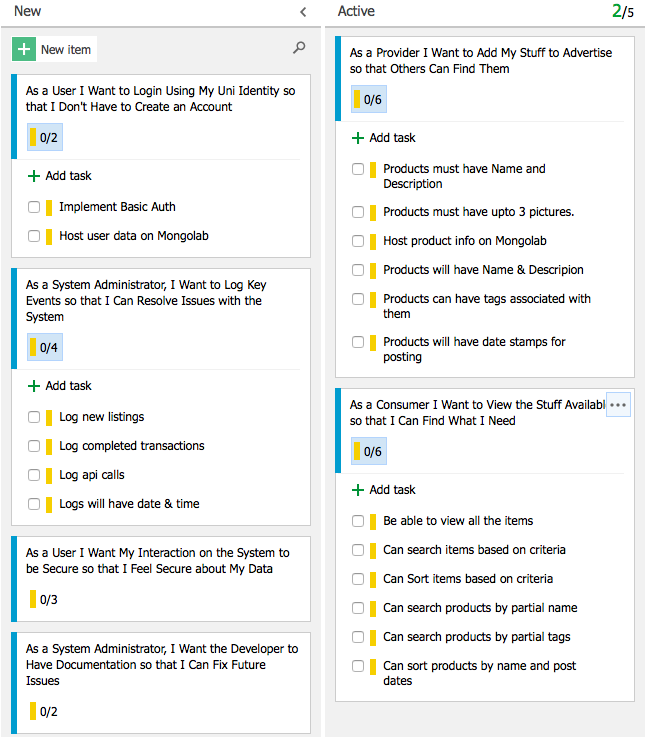
\includegraphics[height = \textwidth, width=\textwidth, keepaspectratio]{backlog_v1}
    \caption{Backlog v1}\label{fig:backlog-v1}
\end{figure}

\section{RE with User Participation}

As planned, I set up interviews with 5 potential users, all UoS students. \textit{Participatory Design} is to invite end users in the designing process of software development. Chapter \ref{chap:user} describes the process and my experiences in detail. In short, my target was to ask the interviewees some open ended questions that will help me better understand their \textit{pain points} and have them draw some wireframes on paper. I used the information gathered to include new user stories and select work for the second sprint.

\section{Intermediate Sprints}

The next stage was to develop the user stories from the updated product backlog (Figure \ref{fig:backlog-v2}) in three sprints. After each sprint, I spent 3-4 days in review to test the \textit{user stories} (\textit{not} development testing) to decide if they can be considered closed (\textit{acceptance criteria}, usually performed by the product owner), updated with more work, be simplified etc. I also recorded the bugs, separate on a physical kanban board.\\

At that point, I also re-prioritised the backlog, so that I could complete the user stories that can have the most effect with the least effort (\textit{impact vs feasibility}). I used both the user interviews and my abilities in required technologies as metrics for this procedure.

\subsection{Sprint 2}

This sprint's targets were as follows - 

\begin{itemize}
	\item A basic user profile functionality.
	\item Adding products, view list of added products and basic search.
	\item Simple logging for each HTTP request.
\end{itemize}

The review was shorter than planned, as the prototype was still quite simple. The updated product backlog can be seen in Figure \ref{fig:backlog-v3}. It introduced a new column - \textit{Disregarded} where I placed the user stories that would not be included in the final version. A progress report was submitted after this sprint.

\begin{figure}[!h]
    \centering
    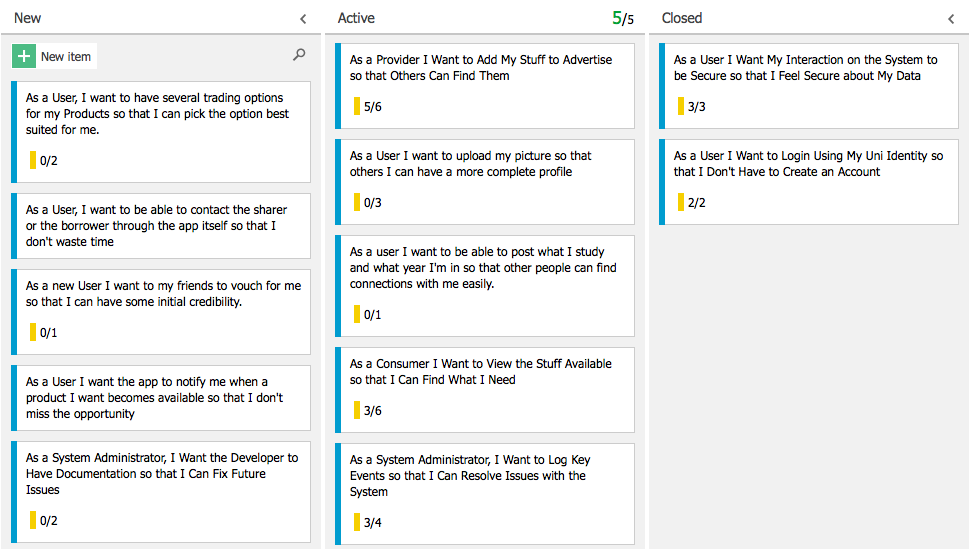
\includegraphics[height = \textwidth, width=\textwidth, keepaspectratio]{backlog_v2}
    \caption{Backlog v2}\label{fig:backlog-v2}
\end{figure}

\subsection{Sprint 3}

The next sprint, performed during the Christmas period, was set to complete user stories regarding - 

\begin{itemize}
	\item Adding some trading options - lend, sell etc.
	\item Allow offers/requests to be made regarding products.
	\item Allow users to accept/decline offers.
\end{itemize}

Another major goal in this iteration was to start formal JavaScript testing, starting from server routes. I discuss about testing in more detail in Chapter \ref{chap:test}. This sprint review revealed two choices for the next sprint - 

\begin{description}
	\item [Chat] functionality between two users.
	\item [Push Notifications] sent regarding offers made on products.
\end{description}

Whereas, every user wanted push notifications for not only offers, but also for several other user stories, chatting only serves a single user story - \textit{in-app communication}. Each required a significant learning curve, and project plan and timings could only accommodate one to be done \textit{well}. I chose notifications, because it could be used in various purposes and allow me to gain better insights into mobile development (\textit{push notifications} being more prevalent on mobile platforms). The updated product backlog can be seen in Figure \ref{fig:backlog-v4}.

\begin{figure}[!h]
    \centering
    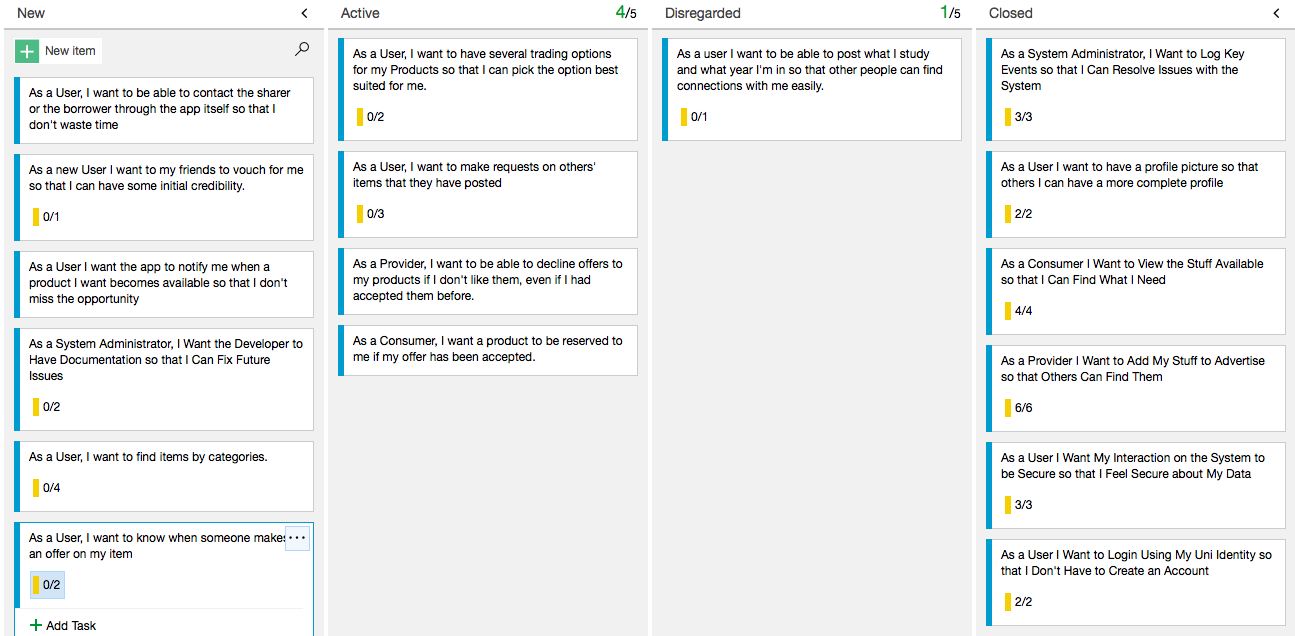
\includegraphics[height = \textwidth, width=\textwidth, keepaspectratio]{backlog_v3}
    \caption{Backlog v3}\label{fig:backlog-v3}
\end{figure}

\subsection{Sprint 4}

As planned, this iteration, starting in the Semester 2, was to finish the user stories already present on the backlog. The primary goal in this iteration was to implement push notifications regarding the offers made on products. Some of the major tasks were - 

\begin{itemize}
	\item Integrate GCM with the server.
	\item Register client device for push notifications.
	\item Send push notifications to the correct users, in time.
\end{itemize}

During the development and review, I realised that push notifications were both unreliable and quite difficult to test. However, I marked the user stories as done by simplifying the acceptance criteria. The next stage was to perform User Experience (UX) evaluation on the current prototype.

\begin{figure}[!h]
    \centering
    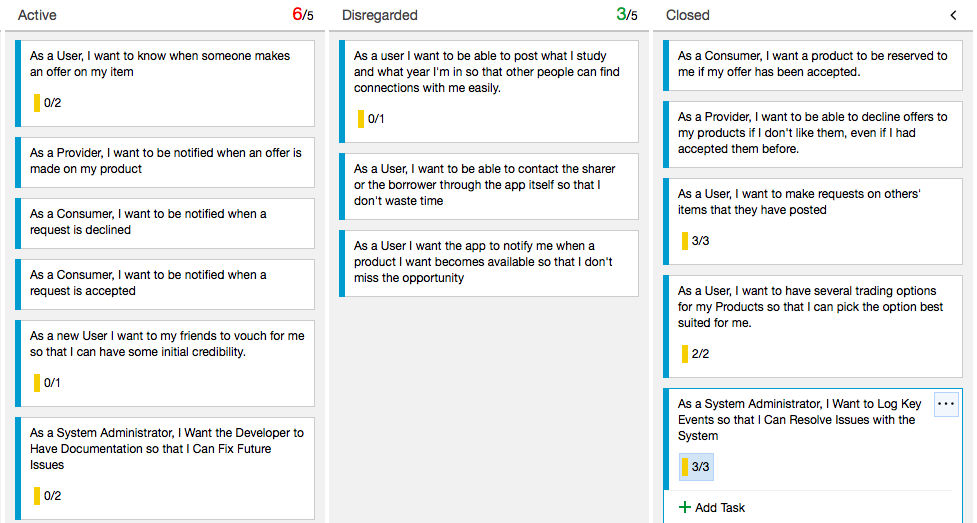
\includegraphics[height = \textwidth, width=\textwidth, keepaspectratio]{backlog_v4}
    \caption{Backlog v4}\label{fig:backlog-v4}
\end{figure}

\begin{figure}[!h]
    \centering
    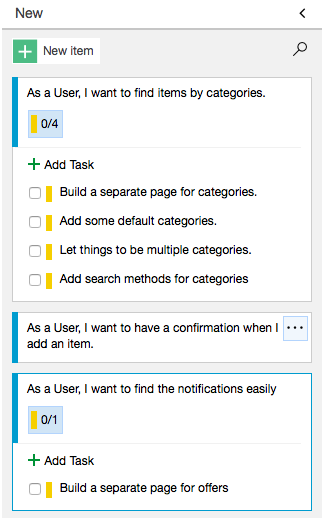
\includegraphics[height = 0.8\textwidth, width=\textwidth, keepaspectratio]{backlog_v5}
    \caption{Final User Stories}\label{fig:backlog-v5}
\end{figure}

\section{UX Evaluation}

Interviews were set up with the same users who were interviewed earlier to evaluate the prototype. I have discussed the process in detail in chapter \ref{chap:user}. The results were largely satisfactory. However, it also gave rise to a number of issues, found in Appendix \ref{appendix:ux}. I evaluated the issues and prioritised them based on effort needed to address them. The final backlog was updated as seen in Figure \ref{fig:backlog-v5}.

\section{Final Sprint}

The final sprint's goal was to resolve most of the simple issues found in the UX evaluation and focus on at least half of the major issues. The results included - 

\begin{itemize}
	\item New app layout to utilise white space better.
	\item Separate sections for categories and offer notifications.
\end{itemize}

In the final sprint review, I found most of my originally planned specifications to be completed to a satisfactory level (for an alpha stage prototype, not a production ready app). So, I discarded the final UX evaluation interviews, which were only planned if significant issues were found in the previous evaluation.

